%% Template for a preprint Letter or Article for submission
%% to the journal Nature.
%% Written by Peter Czoschke, 26 February 2004
%%

\documentclass{nature}
%\documentclass[12pt]{article}

%% make sure you have the nature.cls and naturemag.bst files where
%% LaTeX can find them

\bibliographystyle{naturemag}

\usepackage{graphicx}
\usepackage{amssymb,amsfonts,amsmath}
\usepackage{subfigure}
\usepackage{stfloats}


%% OPTIONAL MACRO DEFINITIONS
\def\s{\sigma}
\newcommand{\be}[0]{\begin{equation}}
\newcommand{\ee}[0]{\end{equation}}
\newcommand{\lb}[0]{\left(}
\newcommand{\rb}[0]{\right)}


\title{Human-induced Arctic sea-ice loss and cold Eurasian winters}

%% Notice placement of commas and superscripts and use of &
%% in the author list


\author{Kelly E. McCusker,*$^{1,2}$ \& John C. Fyfe,$^{2}$ \& Michael Sigmond$^2$}

% NatGeo requirements:
% Title If possible, the title should give a sense of the main new finding, and should not exceed 90 characters, including spaces. Nature Geoscience titles do not contain technical terms or abbreviations unless absolutely necessary. We strongly discourage punctuation or active verbs.@@
% Letter 2,000 words no methods, 3 figures
% Article 3,000 words no methods, include section titles, 6 figures. No refs in abstract. ~500 words of Intro. 1-2 para of conclusions


\begin{document}

\maketitle

\begin{affiliations}
 \item School of Earth and Ocean Sciences, University of Victoria, Victoria, BC, V8P 5C2, Canada
 \item Canadian Centre for Climate Modelling and Analysis, Environment Canada, Victoria, BC V8W 2Y2, Canada
\end{affiliations}


\begin{abstract}
Arctic sea ice loss has been implicated in the recent trend toward unusually cold Eurasian winters \cite{liu12,mori14,kim14}. Whether the linkage follows from anthropogenic sea ice loss, however, remains an open question as the sea-ice loss combines anthropogenic response and internal (random) variability \cite{swart15,wettstein14} and because of confounding wintertime variability over the Eurasian continent \cite{deser12b,screen14a}. Here, we isolate the anthropogenic and random components of the linkage using a large ensemble of atmosphere-only model simulations with prescribed sea ice loss taken from simulations of the companion atmosphere-ocean-cryosphere model and from observations. We find no evidence of a sea-ice loss related decrease in Eurasian winter temperature. However, we do find long periods of winter Eurasian cooling linked to internally-generated circulation features over the Barents and Kara Seas regions of the Arctic. These results challenge the perception that Arctic sea ice loss was responsible for the recent prevalence of unusually cold Eurasian winters, showing instead that these winters were more likely the consequence of internal variability, with implications for our understanding of impacts and adaptation in human and natural high-northern latitude systems. 
\end{abstract}

Global average surface air temperatures in the boreal cold season have been rising faster than the annual average \cite{wallace12} and exhibit further enhanced warming over the Arctic in part due to positive feedbacks related to sea-ice loss \cite{screen10,cohen14}. Epoch differences of winter (December-January-February; DJF) surface air temperature (SAT) between 2002-12 and 1979-89 reveal warming upward of 2$^\circ$C over the polar cap, collocated with areas of sea ice loss (Figure \ref{fig:fig1}a). Contemporaneous cooling of greater than 1$^\circ$C over the Eurasian continent in winter is also evident; a feature that is particularly striking when considered in the context of broad hemispheric warming, which can in part be attributed to anthropogenic forcing \cite{gillett08,qian15}. 

Since the year 2000, there have been a greater number of Eurasian winters exhibiting increasingly cold anomalies, especially in relation to the evolution of northern hemisphere temperature; Figure \ref{fig:fig1}b shows Eurasian winter SAT with northern hemisphere average temperature removed. Coincident with these cold anomalies, large reductions in autumn and winter Arctic sea ice area have occurred, particularly in the Barents and Kara Seas (BKS) sector (along the western half of the Russian coastline; Figure \ref{fig:fig1}c). Observationally-based regression and composite analyses confirm that there is a positive correlation between BKS sea ice concentration and Eurasian SAT \cite{inoue12,outten12}, although causation between sea-ice and Eurasian SAT cannot be established with observations alone. Model evidence supports this connection through a Rossby wave-train emanating out of the BKS region, incited by turbulent heat flux from the increased area of open water \cite{honda09,petoukhov10,mori14,kim14,peings14}. However, while human influence on observed Arctic sea ice extent is clear \cite{min08}, interpretation of this Arctic sea ice--Eurasian SAT connection as an anthropogenic signal is limited by the strong imprint of internal variability on observed sea ice loss itself \cite{swart15}. 

To estimate the anthropogenic component of observed winter sea-ice loss, we examine a distribution of DJF sea ice loss between the periods (1979-89) and (2002-12) in a large ensemble (LE) of 50 Historical simulations executed in the Canadian Earth System model version 2 (CanESM2; Figure \ref{fig:fig2}). The average of the distribution represents the anthropogenically-forced sea ice area anomaly, while each individual realization represents one version of an ``observation", displaced from the average by some amount due only to internally-generated variability. Here internal variability generates a range in DJF sea ice loss over this time period of approximately 1 million km$^2$. 

An estimated upper bound on the contribution of internal variability to a sea-ice area anomaly can be made using the extreme end-points of the distribution in Figure \ref{fig:fig2}: taking the minimum ice anomaly (-1.7e$^6$ km$^2$) distance from the distribution average (-1.2e$^6$ km$^2$), we find that internal variability can account for up to 40\% of the historical sea-ice area anomaly: (-1.7e$^6$ - (-1.2e$^6$))/-1.2e$^6$ = 0.39 or about 40\%. Similarly, the maximum ice anomaly (-0.7e$^6$ km$^2$) gives approximately 40\%. The true observed DJF Arctic sea-ice area anomaly derived from satellite measurements by the National Snow and Ice Data Center (NSIDC) is encompassed by the Historical LE (Figure \ref{fig:fig2}) and indicates a similar contribution from internal variability (36\%), somewhat smaller than alternative calculations that equal 47-57\% for September sea ice trends \cite{kay11,stroeve07}. Thus by our estimate, at least 60\% of the magnitude of winter sea ice loss is likely anthropogenically-forced. 

Next we isolate the effect of human-induced Arctic sea ice loss on the atmosphere by executing a large ensemble of Canadian atmosphere general circulation model (CanAM4) simulations in which prescribed ``past" (1979-89) and ``present-day" (2002-12) boundary conditions are taken from an average of five CanESM2 Historical simulations (Figure \ref{fig:fig2} and Supplementary Figure 1) that were submitted to the Climate Model Intercomparison Project 5 (CMIP5). These average boundary conditions represent an estimate of the human-induced component by averaging out internal variability. 

A set of five 120-year AGCM simulations, differing only in initial conditions, is executed with annually-repeating, monthly sea-ice concentration (SIC), sea-ice thickness (SIT), and sea surface temperature (SST) for ``past" boundary conditions and for ``present-day" boundary conditions in which only Arctic SIC, SIT, and Arctic SST (where SIC $<$ 15\% in the present day but not the past) are set to present-day climatologies. All else is set to past climatologies. Atmospheric constituents are set to 1984 values for all simulations (see Methods). The anomalies between these past and present-day simulations, known as the ``Average SIC forcing" ensemble, estimate the isolated response of the atmosphere to human-induced sea ice loss. We similarly execute five pair of 120-year AGCM simulations with boundary conditions taken from the five individual CanESM2 Historical simulations (``Individual SIC forcing" ensemble) to represent the response to varying boundary conditions in which internal variability is incorporated. Thus in total, each ensemble consists of 600 years of (present - past) anomalies. In addition, we execute a pair of 120-year simulations with past and present-day NSIDC boundary conditions (Figure \ref{fig:fig2} and Supplementary Figure 1).

We first present the responses of regionally-averaged winter SAT anomalies from all simulations as ``uncertainty cascades" \cite{wilby10,swart15}, where uncertainty is based on the number of simulation years averaged (Figure \ref{fig:fig3}). This presentation demonstrates the powerful influence of internal variability in response to a forcing. A reduction in SIC reveals newly open seawater that provides a source of heat to the atmosphere. As such, the local effect of human-induced sea ice loss, averaged across the Average SIC forcing ensemble (600-year average), is a warming over the polar cap (averaged north of 60$^\circ$N) of just over 1$^\circ$C in winter (Figure \ref{fig:fig3}a). When evaluating 120-year averages instead, a spread in responses that ranges from $~$0.9$^\circ$C to 1.3$^\circ$C is evident, with the spread across 60-year averages wider still. 

These spreads are noteworthy because the boundary conditions for each 120-year and 60-year average are identical, indicating that the range of anomalies must be due solely to internal variability even at these large sample sizes. Furthermore, the range of 120-year and 60-year average SAT responses in the Individual SIC forcing ensemble (Figure \ref{fig:fig3}a) are comparable to those of the Average SIC forcing ensemble, indicating that even local, polar-cap, sensitivity of SAT to varied sea ice loss conditions is overpowered by internal variability in winter. The polar cap SAT response to NSIDC SIC boundary conditions is also about 1$^\circ$C (Figure \ref{fig:fig3}a), consistent with the modelled boundary conditions.   

Given the polar cap results, it should perhaps come as no surprise that results outside the Arctic are more variable and less robust. The SAT response over Eurasia is not statistically different from zero in either the Individual or Average SIC forcing ensemble averages, demonstrating that the robust response of Eurasian winter temperature to human-induced Arctic sea-ice loss is not cooling, but rather there is no signal (Figure \ref{fig:fig3}b). Individual 120-year and 60-year average anomalies are generally not significant (90\% level) and span zero in both SIC forcing ensembles. Nevertheless, some 120-year and 60-year average anomalies show statistical significance, most notably the 60-year average cooling associated with NSIDC SIC forcing that is not robust to the 120-year average. This point is important to recognize because many studies understandably utilize 60- to 100-year integrations or ensembles to draw conclusions that may prove inaccurate given larger ensemble sizes.

Arctic sea ice loss can yield either warmer or cooler Eurasian SAT in winter (Figure \ref{fig:fig3}b). To understand this further, we examine the spatial pattern of circulation associated with the warmest and coldest cases in the Average SIC forcing ensemble (Figure \ref{fig:fig4}), in which boundary conditions are identical and each average has a sample size of 120 years. The patterns of geopotential height at 500 hPa (Z500) in the two cases are distinct, and in some locations such as over the BKS, nearly opposite. The cooling case (Figure \ref{fig:fig4}a) shows a zonally-symmetric increase in Z500 to the north and a weak decrease over central Eurasia. This pattern is conducive for advection of polar air to the south and west along Z500 contours. In contrast, the warming case (Figure \ref{fig:fig4}b) exhibits an azonal pattern with a decrease in Z500 over the BKS region and increases over the southern continent and the northeast. This pattern favours warm-moist air advection from the south and west. Thus, the response of Eurasian SAT is consistent with thermal advection due to internally-varying circulation patterns. 

The relationship between the winter circulation over the Barents-Kara Seas and Eurasian SAT is genuine and exists across 120-year average anomalies, including the response to observed (NSIDC) SIC boundary conditions (Figure \ref{fig:fig5}). As Z500 anomalies over the Barents-Kara Seas increase, Eurasian SAT anomalies robustly decrease (r$^2$=0.72; p=0.002). The same relationship exists inter-annually between anomalies within each individual simulation pair in time (0.36 $<$ r$^2<$ 0.50; p $<$ 0.001). Thus, the physical mechanisms that lead to the Eurasian cooling case are consistent with existing work that implicates high geopotential heights over the Barents-Kara Seas region \cite{honda09,petoukhov10,mori14}. What is novel here, however, is that there is no indication that changes in sea-ice concentration are the fundamental origin of Eurasian SAT anomalies because sea-ice concentration is prescribed in our simulations. 

In further support of the insignificance of the sea ice boundary forcing for Eurasian SAT, we find no relationship between 120-year average BKS net surface fluxes (latent, sensible, and downwelling longwave fluxes) and Eurasian SAT (r$^2$=0.11; p=0.35), or BKS SAT and Eurasian SAT (r$^2$=0.13; p=0.31). Moreover, simulations with present-day sea ice do not exhibit a greater frequency of anomalously cold Eurasian SAT in winter compared to simulations with past sea-ice conditions.

We have seen that neither human-induced sea-ice loss, nor observed sea-ice loss consistently causes Eurasian cooling in our simulations. Rather internal variability, even with a sample of 120 years, is the dominant effect because there is effectively no signal in winter over Eurasia. This result is not sensitive to the definition of the Eurasian region or to the choice of winter months considered. What, then, is the cause of Eurasian winter cooling in the observational record? Others have suggested changes in the North Atlantic SST \cite{sato14}, or increased blocking due to the phase of the Atlantic Multidecadal Oscillation and North American Oscillation \cite{peings14b}, both manifestations of internal variability in the climate system. 

The CanESM2 Historical LE provides a rich resource in which observations --- one outcome of historical forcing and internal variability --- can be put into the context of many other potential outcomes. The LE exhibits a relationship across its ensemble members between winter BKS Z500 and Eurasian SAT anomalies (present - past) that compares well with that shown in Figure \ref{fig:fig5}, but with greater variability due to the 11-year averaging periods (Supplementary Figure 2). In addition, there is a weak but significant negative correlation in the LE between Barents-Kara Seas sea-ice concentration and the Z500 anomaly overhead (more SIC loss is associated with larger positive height anomalies; r=-0.28; p=0.05), but notably there is no linkage between BKS SIC and Eurasian SAT (r=-0.03; p=0.8). This provides evidence that surface conditions in the Barents-Kara Seas can influence geopotential heights overhead, consistent with previous studies \cite{honda09,mori14}, but the height anomalies are too weak to produce an identifiable anomaly, cold or warm, in Eurasia (Supplementary Figures 3 and 4). 

Observed geopotential height over the Barents-Kara Seas and observed SAT over Eurasia (obtained from ERA-Interim and GIStemp, respectively; see Methods) fall within the LE distribution, when NH SAT is removed to account for any biases in the modelled hemispheric SAT response to historical forcing (Supplementary Figure 2). Thus, Z500 anomalies that are associated with Eurasian cooling are explained by internal variability, in agreement with the AGCM results. We show through multiple lines of evidence that sea-ice loss in the Barents and Kara Seas has a discernible impact on local climate but limited influence on Eurasian winter climate because of a lack of robust, large-scale circulation changes due to sea ice loss, human-induced or otherwise. Rather, circulation changes associated with Eurasian climate are internally-generated.  


\begin{methods}
\textbf{Observations} \\
blah blah blah
\\
\textbf{Model simulations}\\
blah
\end{methods}

\begin{figure}%[htbp] % the star afterwards makes it a one column fig in a 2-col document
\centering
\noindent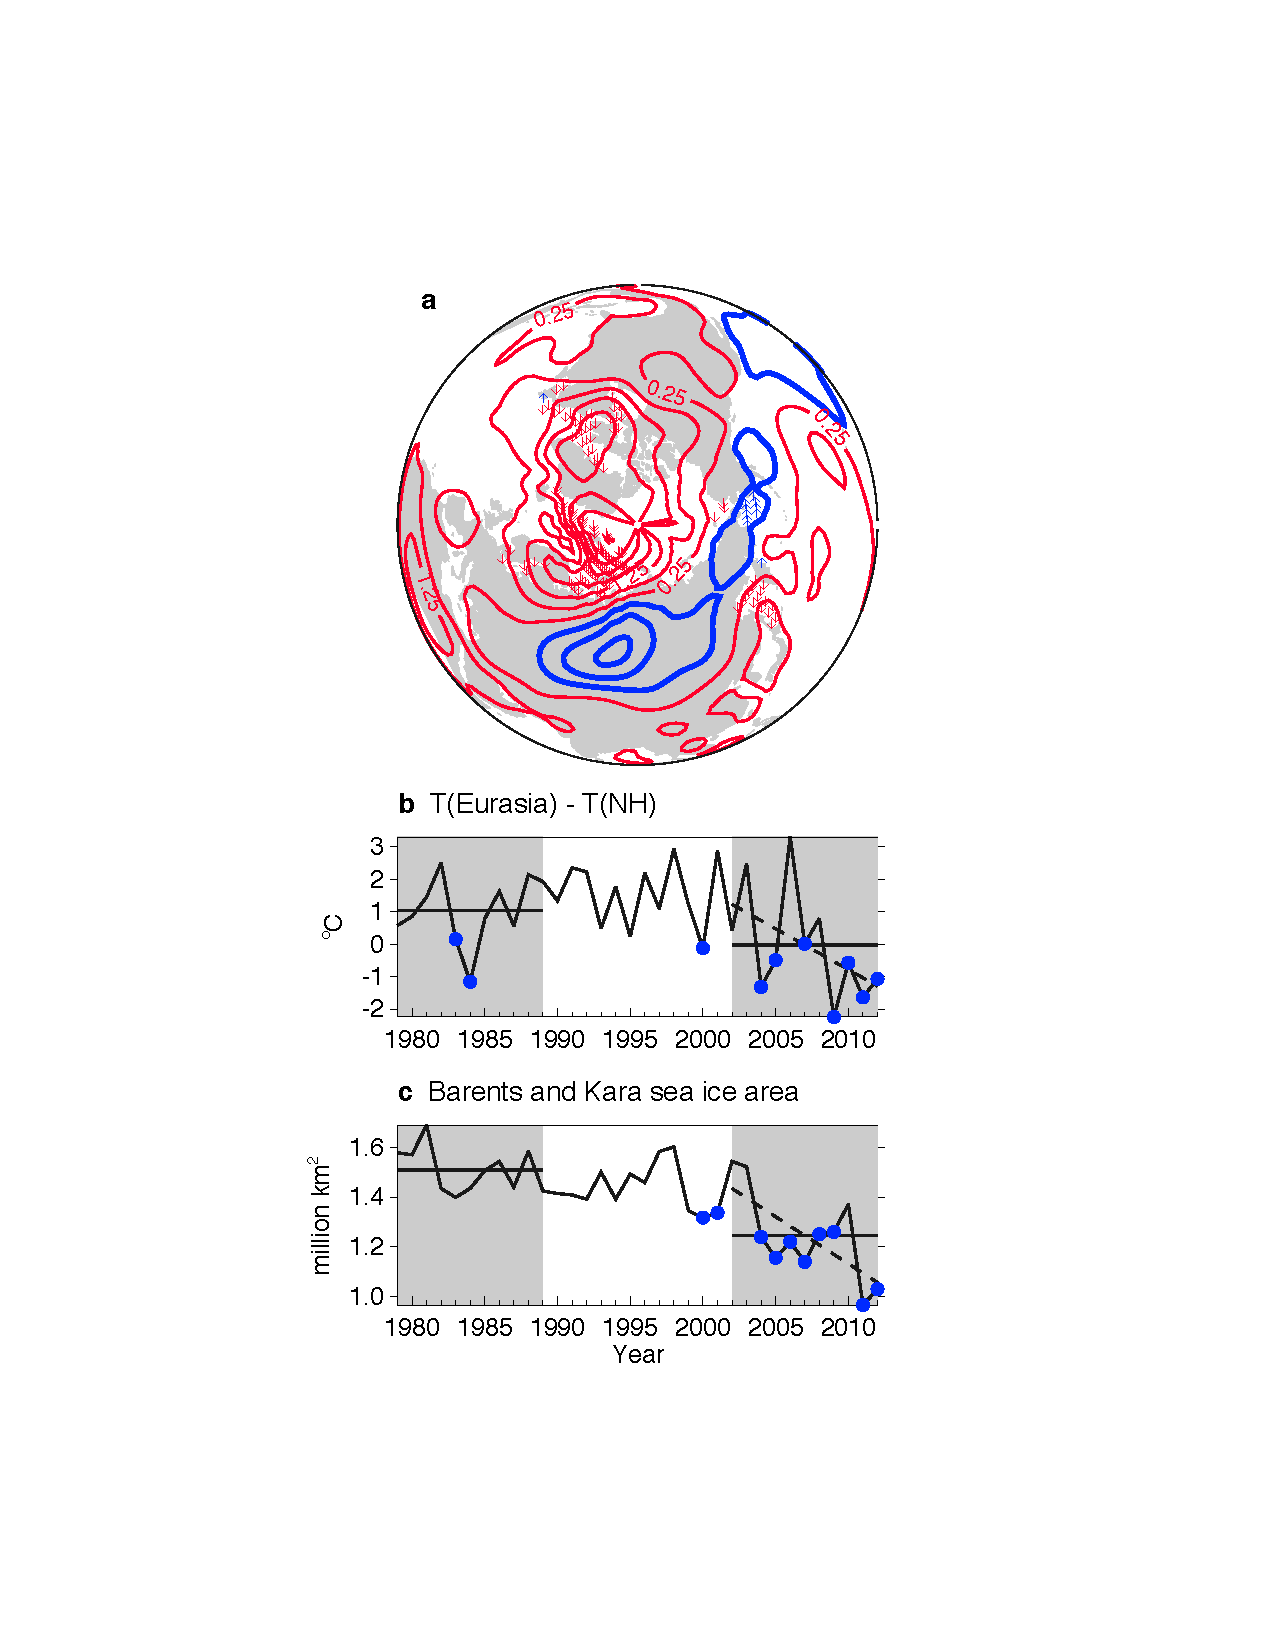
\includegraphics[width=19pc]{PLOT1.pdf}
\caption{\textbf{Observed surface air temperature and sea ice concentration.} a.) Map of GIStemp winter surface air temperature anomalies as (2002-12) minus (1979-89) in contours. Contour interval is 0.5$^\circ$C with zero contour omitted. Arrow markers indicate regions of sea ice loss (red) and gain (blue) that are greater than 40\% in absolute terms. b.) Time series of Eurasian-averaged (35$^\circ$N - 60$^\circ$N, 40$^\circ$E - 120$^\circ$E) winter SAT with hemispheric (NH) winter temperature removed. Blue markers indicate the 10 most negative anomalies since 1979. c.) Time series of Barents-Kara Seas region (65$^\circ$N - 80$^\circ$N, 27$^\circ$E - 96$^\circ$E) winter sea ice area. Blue markers indicate the 10 lowest concentrations since 1979.
}
\label{fig:fig1} 
\end{figure}

\begin{figure}%[htbp] % the star afterwards makes it a one column fig in a 2-col document
\centering
\noindent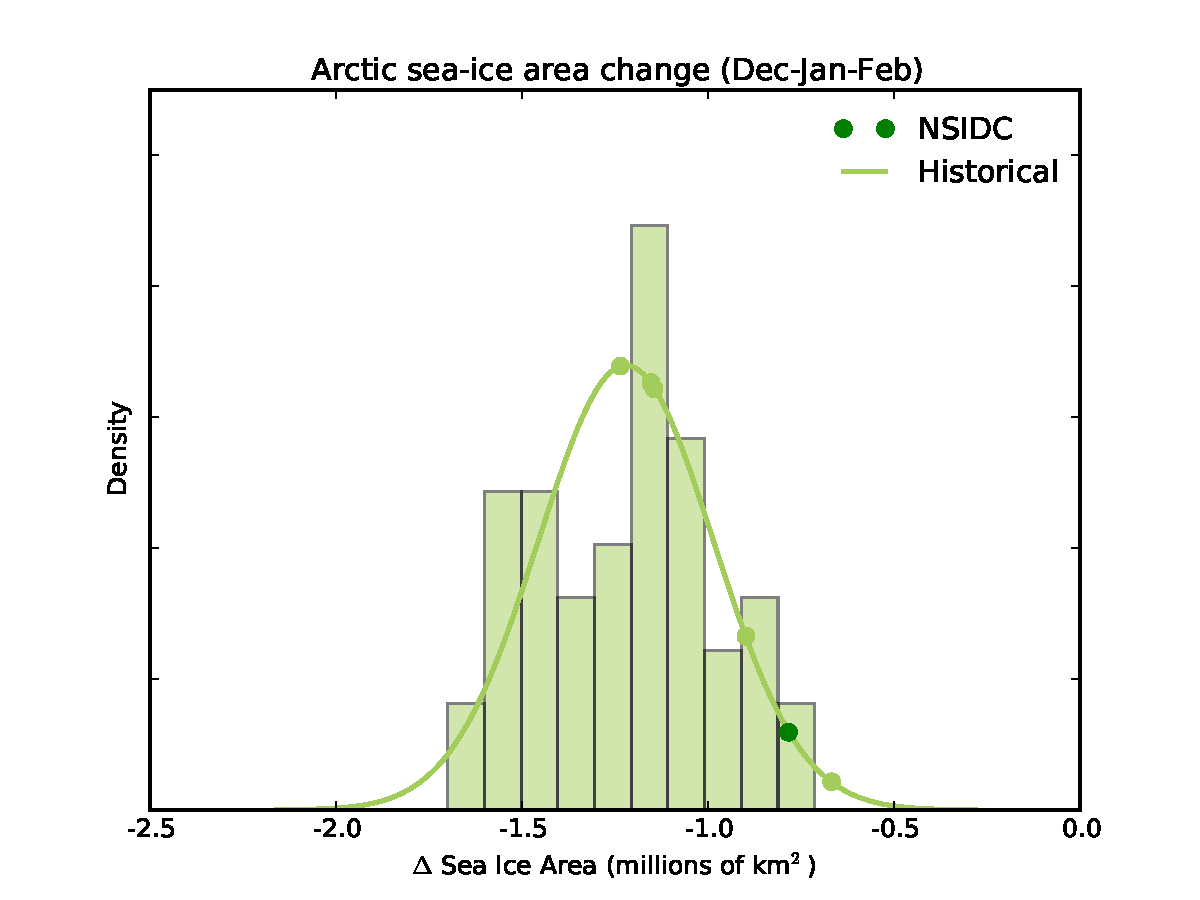
\includegraphics[width=25pc]{Figure2b.pdf}
\caption{\textbf{CanESM2 large ensemble change in winter sea ice area.} Histogram and histogram fit of winter averaged Arctic sea-ice area changes from the period 1979-89 to 2002-12 in the CanESM2 Historical large ensemble (50 members). Light green markers indicate the original five Historical simulations, published as part of CMIP5 and seeds for the Historical LE, and also prescribed as boundary conditions to our `Individual SIC forcings' AGCM simulations. The average of these 5 markers is the boundary condition to our `Average SIC forcing' AGCM simulations. The dark green marker shows Arctic sea-ice change from the NSIDC bootstrap observational dataset. Filled markers indicate the present day period (2002-12) is significantly different from the past (1979-89) at the 90\% level using the Student’s T test of difference between two means. 
}
\label{fig:fig2} 
\end{figure}

\begin{figure}%[htbp] % the star afterwards makes it a one column fig in a 2-col document
\centering
\noindent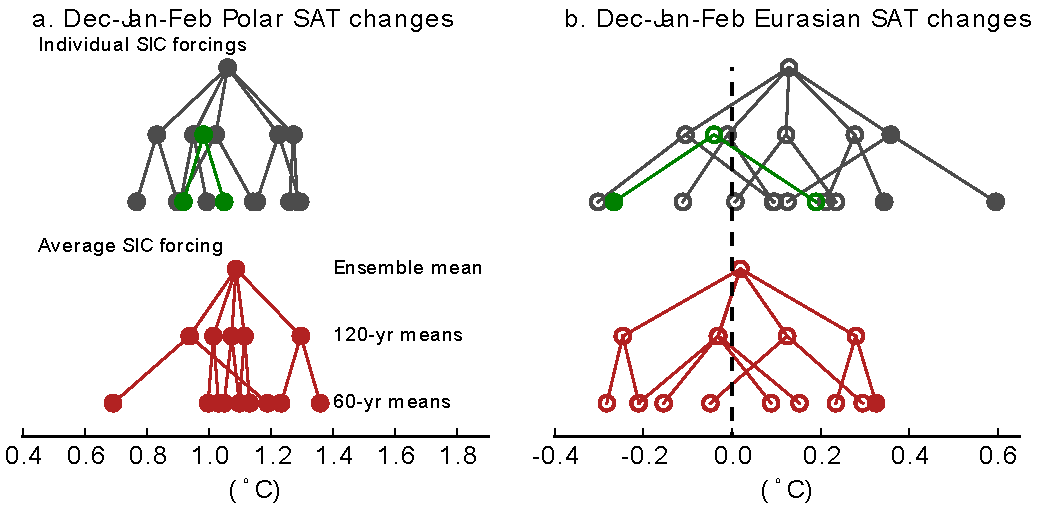
\includegraphics[width=35pc]{Figure3.pdf}
\caption{\textbf{Simulated polar cap and Eurasian temperature response uncertainty cascades.} Regional winter response of SAT to Individual SIC forcings (black) and Average SIC forcing (red) shown as uncertainty cascades of the a.) polar cap anomalies (averaged poleward of 60$^\circ$N) and b.) Eurasian anomalies (averaged within 35$^\circ$N - 60$^\circ$N, 40$^\circ$E - 120$^\circ$E). Each cascade consists of the ensemble average of five 120-year ensemble members (top level), individual 120-year ensemble member averages (middle level), and ensemble members sub-sampled into two 60-year segment averages (bottom level). Filled circles indicate significance at the 90\% level using the Student’s T test of difference between two means. 
}
\label{fig:fig3} 
\end{figure}

\begin{figure}%[htbp] % the star afterwards makes it a one column fig in a 2-col document
\centering
\noindent\includegraphics[width=39pc]{Figure4_orSuppFig2.pdf}
\caption{\textbf{Winter surface air temperature and geopotential height responses.} Winter average SAT anomaly ($^\circ$C) with geopotential height at 500 hPa anomalies in contours (contour interval = 3m) for c) \textit{should be a)} the Average SIC forcing ensemble member with the coldest Eurasian SAT anomaly, and for d) \textit{should be b)} the Average SIC forcing ensemble member with the warmest Eurasian SAT anomaly.
}
\label{fig:fig4} 
\end{figure}

\begin{figure}%[htbp] % the star afterwards makes it a one column fig in a 2-col document
\centering
\noindent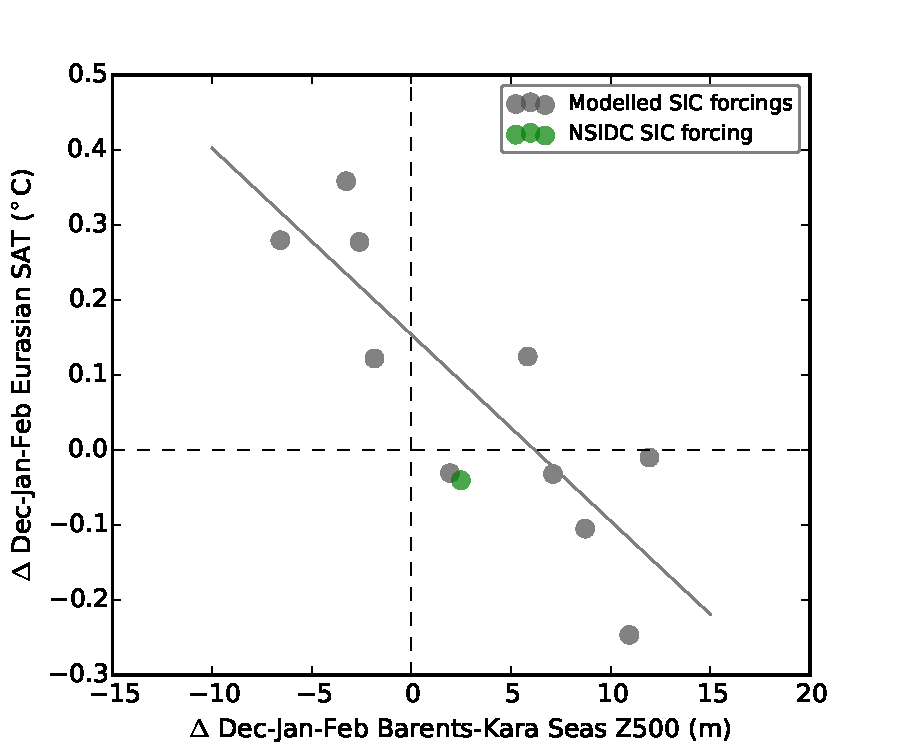
\includegraphics[width=25pc]{Figure5.pdf}
\caption{\textbf{Winter Eurasian surface air temperature versus Barents-Kara geopotential height.} Winter averaged Eurasian SAT ($^\circ$C) versus geopotential height at 500 hPa over the Barents-Kara Seas region (65$^\circ$N - 80$^\circ$N, 27$^\circ$E - 96$^\circ$E). Grey circles indicate 120-year average anomalies for each member of the Individual and Average SIC forcing ensembles, shown together because the distributions are statistically indistinguishable from one another (mean and variance of BKS Z500 and Eurasian SAT between the two ensembles are not different). The dark green marker indicates the 120-year average anomaly from the NSIDC SIC forcing simulation pair. The regression line ($r^2$ = 0.72, $p$ = 0.002) does not include the NSIDC SIC forcing simulation average.
}
\label{fig:fig5} 
\end{figure}

\begin{figure}%[htbp] % the star afterwards makes it a one column fig in a 2-col document
\centering
\noindent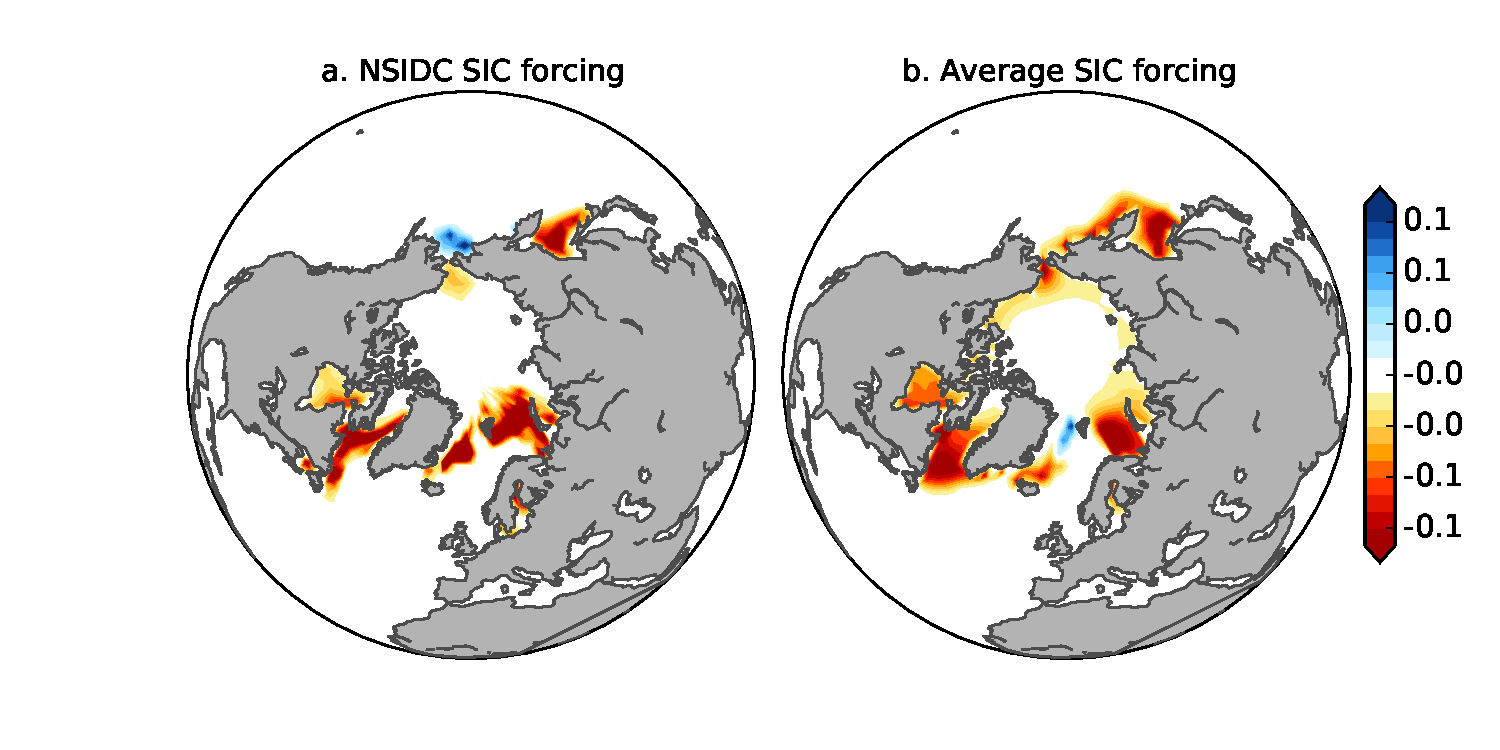
\includegraphics[width=30pc]{SuppFigure1.pdf}
\caption{\textbf{Supplementary Figure 1. Maps of SIC forcing in winter.} a.) Winter sea ice concentration (fraction) boundary forcing for the NSIDC simulations, derived from the NSIDC bootstrap dataset. Anomalies are (2002-11) minus (1979-89). b.) is as (a) except for the boundary forcing averaged from the five CanESM2 historical ensemble members. Anomalies are (2002-12) minus (1979-89).
}
\label{fig:supp1} 
\end{figure}

\begin{figure}%[htbp] % the star afterwards makes it a one column fig in a 2-col document
\centering
\noindent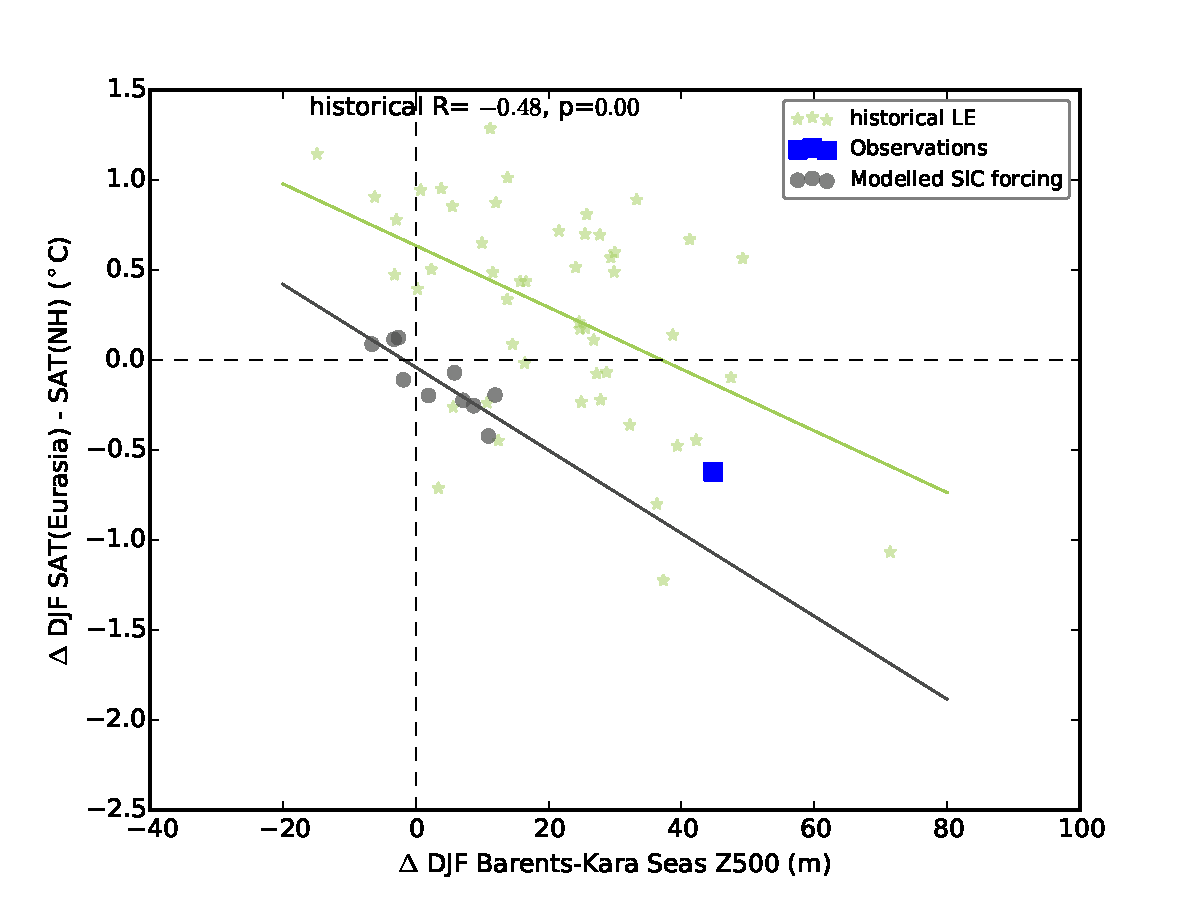
\includegraphics[width=25pc]{SuppFigure2_nhremoved_simsadded.pdf}
\caption{\textbf{Supplementary Figure 2. CanESM2 Historical Large Ensemble winter Eurasian-NH SAT and BKS Z500 anomalies.} Eurasian SAT shown with northern hemisphere temperature removed, to normalize against temperature bias in the Historical LE, plotted against Z500 over the Barents-Kara Seas (BKS) region. Values are shown as anomalies (2002-12 minus 1979-89) from the 50 Historical LE members (green), observations from ERA-Interim for Z500 and GIStemp for SAT (blue), and as 120-year averages from the SIC forcing simulations (as in Figure 5 in the main text). The regression slope for the Historical LE is -0.17$^\circ$C/10 m, $p <$ 0.001. Simulated 120-year averages give a regression slope of -0.23$^\circ$C/10 m, $p$ = 0.002. Recall that the LE encompasses the response to all historical radiative forcings whereas the SIC forcing simulations show the isolated response to sea-ice loss. Further, LE and observed data points are differences of 11-year means, whereas the SIC forcing simulations exhibit significantly less scatter due to the long time average of 120 years. These two effects explain the generally greater magnitudes of Eurasian SAT and Z500 anomalies in the LE and observations compared with SIC forcing simulations.
}
\label{fig:supp2b} 
\end{figure}

\begin{figure}%[htbp] % the star afterwards makes it a one column fig in a 2-col document
\centering
\noindent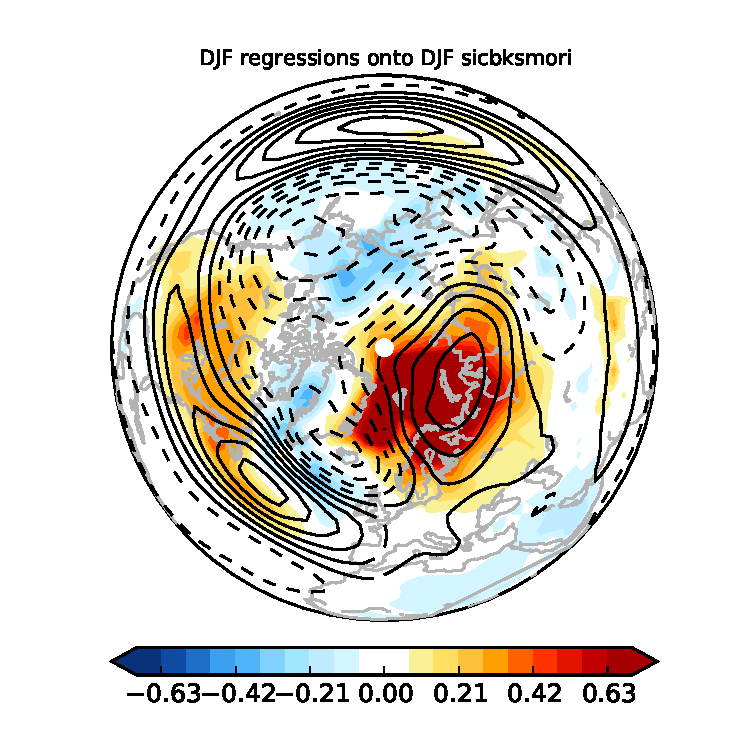
\includegraphics[width=25pc]{SuppFigure3.pdf}
\caption{\textbf{Supplementary Figure 3. CanESM2 Historical Large Ensemble regressions on BKS SIC.} \textit{[This figure is a draft.]} Regression of winter SAT (color) and winter Z500 (contours) onto normalized BKS SIC and multiplied by -1 such that positive temperature and height anomalies are associated with sea ice loss. Z500 contour interval starts at +/- 0.67 m per $\sigma$ in BKS SIC, with contour interval 1.33 m/$\sigma$. There is no zero line.
}
\label{fig:supp3} 
\end{figure}


\begin{figure}%[htbp] % the star afterwards makes it a one column fig in a 2-col document
\centering
\noindent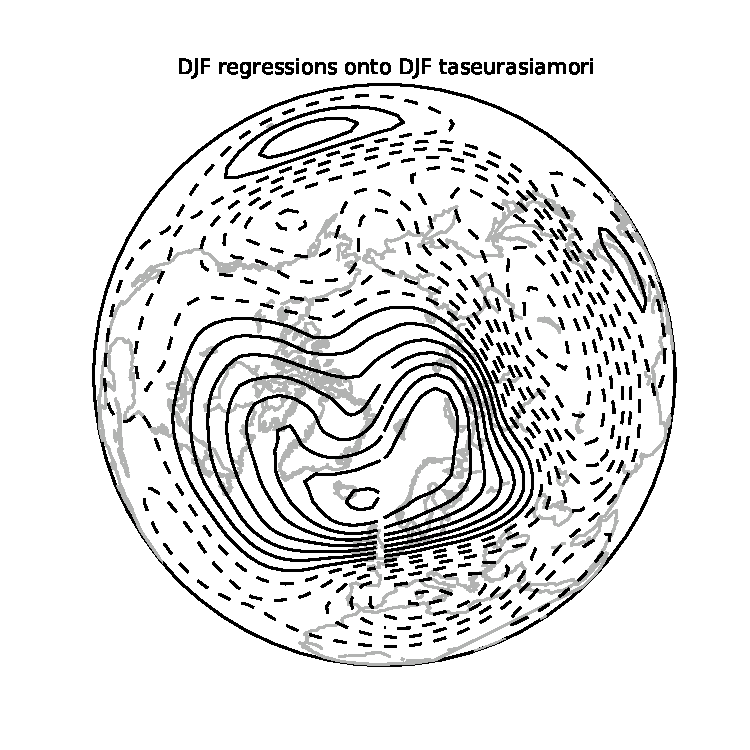
\includegraphics[width=25pc]{SuppFigure4.pdf}
\caption{\textbf{Supplementary Figure 4. CanESM2 Historical Large Ensemble Z500 regression on Eurasian SAT.} \textit{[This figure is a draft.]} Regression of winter Z500 onto normalized Eurasian SAT and multiplied by -1 such that positive height anomalies are associated with negative Eurasian SAT anomalies. Z500 contour interval starts at +/- 0.67 m per $\sigma$ in Eurasian SAT, with contour interval 1.33 m/$\sigma$. There is no zero line.
}
\label{fig:supp4} 
\end{figure}

%% Put the bibliography here, most people will use BiBTeX in
%% which case the environment below should be replaced with
%% the \bibliography{} command.

%\begin{thebibliography}{1}
%\end{thebibliography}
\newpage

%\bibliographystyle{ametsoc}
\bibliography{allrefs}





% ~/bibtexrefs/allrefs  == this is version controlled now, but will have to just copy into current dir?


%% Here is the endmatter stuff: Supplementary Info, etc.
%% Use \item's to separate, default label is "Acknowledgements"

\begin{addendum}
\item[Acknowledgements] 
\item[Author Contributions] 
 \item[Competing Interests] The authors declare that they have no competing financial interests.
\item[Correspondence] Correspondence and requests for materials should be addressed to K.E.M.~(email: kemccusk@uvic.ca).
\end{addendum}

%%
%% TABLES
%%
%% If there are any tables, put them here.
%%

\end{document}
